% Mid-term presentation. Build on the server:
%   python presentation/midterm/make_figures.py      (figures + numbers from the real results)
%   cd presentation/midterm && latexmk -pdf slides.tex
\documentclass[aspectratio=169,11pt]{beamer}
\usetheme[progressbar=frametitle,numbering=fraction,sectionpage=none]{metropolis}
\usepackage{graphicx,booktabs,tabularx,xcolor}
\usepackage[normalem]{ulem}
\usepackage{tikz}
\usetikzlibrary{arrows.meta,positioning,calc,fit,backgrounds}
\usepackage{appendixnumberbeamer}
\graphicspath{{assets/}}

% ---- colours -------------------------------------------------------------
\definecolor{accent}{HTML}{2B6CB0}
\definecolor{accentdark}{HTML}{1A3E6E}
\definecolor{softgrey}{HTML}{A0AEC0}
\definecolor{ink}{HTML}{1A202C}
\definecolor{muted}{HTML}{4A5568}
\definecolor{done}{HTML}{2F855A}
\definecolor{running}{HTML}{B7791F}
\definecolor{nextc}{HTML}{718096}
\definecolor{dropc}{HTML}{C53030}
\definecolor{paper}{HTML}{F7F9FC}
\setbeamercolor{frametitle}{bg=accentdark,fg=white}
\setbeamercolor{progress bar}{fg=accent,bg=accent!20}
\setbeamercolor{normal text}{fg=ink}
\setbeamercolor{alerted text}{fg=accent}
\setbeamerfont{frametitle}{size=\large}

% ---- small helpers -------------------------------------------------------
% plain box (not a nested tikz picture, which inherits sizes when used inside tikz nodes)
\newcommand{\chip}[2]{{\setlength{\fboxsep}{2pt}\colorbox{#1}{\textcolor{white}{\scriptsize\bfseries\strut #2}}}}
\newcommand{\keep}[1]{\item #1}
\newcommand{\dropped}[2]{\item {\color{softgrey}\sout{#1}}\ {\color{dropc}\scriptsize[#2]}}
\newcommand{\bignum}[2]{{\color{accent}\fontsize{19}{21}\selectfont\bfseries #1}\\[-2pt]{\footnotesize\color{muted}#2}}
\newcommand{\muted}[1]{{\color{muted}#1}}
\newcommand{\thumb}[3]{\begin{minipage}[t]{0.31\linewidth}\centering
  \includegraphics[height=2.05cm]{#1}\\[-1pt]{\scriptsize\bfseries #2}\\[-3pt]{\tiny\muted{#3}}\end{minipage}}
\newcommand{\bt}[3]{\begin{minipage}[t]{0.235\linewidth}\centering\includegraphics[width=\linewidth]{#1}\\[2pt]
  {\scriptsize\bfseries #2}\\[-1pt]{\tiny\muted{#3}}\end{minipage}}

\newcommand{\nMunis}{853}
\newcommand{\nCells}{575k}
\newcommand{\nCaptions}{10,000}
\newcommand{\nKept}{84\%}
\newcommand{\nHybridR}{0.52}
\newcommand{\nNtlR}{0.27}
\newcommand{\nBuildings}{10M}
\newcommand{\RQone}{no clear effect ($\Delta$RMSE +0.007, 95\% CI [-0.028, +0.041])}
\newcommand{\RQfour}{V10 better ($\Delta$RMSE -0.028, 95\% CI [-0.050, -0.008])}

\newcommand{\bcapnameA}{Forest}\newcommand{\bcapA}{A predominantly forested area with patches of cleared land.}
\newcommand{\bcapnameB}{Farmland}\newcommand{\bcapB}{A large, circular area of brown farmland, likely recently plowed, dominating the center.}
\newcommand{\bcapnameC}{Village edge}\newcommand{\bcapC}{A sparsely built area with scattered houses and small buildings, likely residential.}
\newcommand{\bcapnameD}{Town centre}\newcommand{\bcapD}{A densely built-up area with numerous houses featuring red-tiled roofs, indicating a residential neighborhood.}


\title{Estimating municipal GDP from satellite embeddings, text and night lights}
\subtitle{Text- and night-light-guided satellite embeddings for regional economic estimation}
\author{Hemant}
\institute{Term project \textbullet\ mid-term review}
\date{October 2026}

\begin{document}

% ==== 1. Title ==============================================================
{\setbeamercolor{background canvas}{bg=white}
\begin{frame}[plain]
\begin{tikzpicture}[remember picture,overlay]
  \node[anchor=east,inner sep=0] (map) at ($(current page.east)+(-0.3,0.25)$)
    {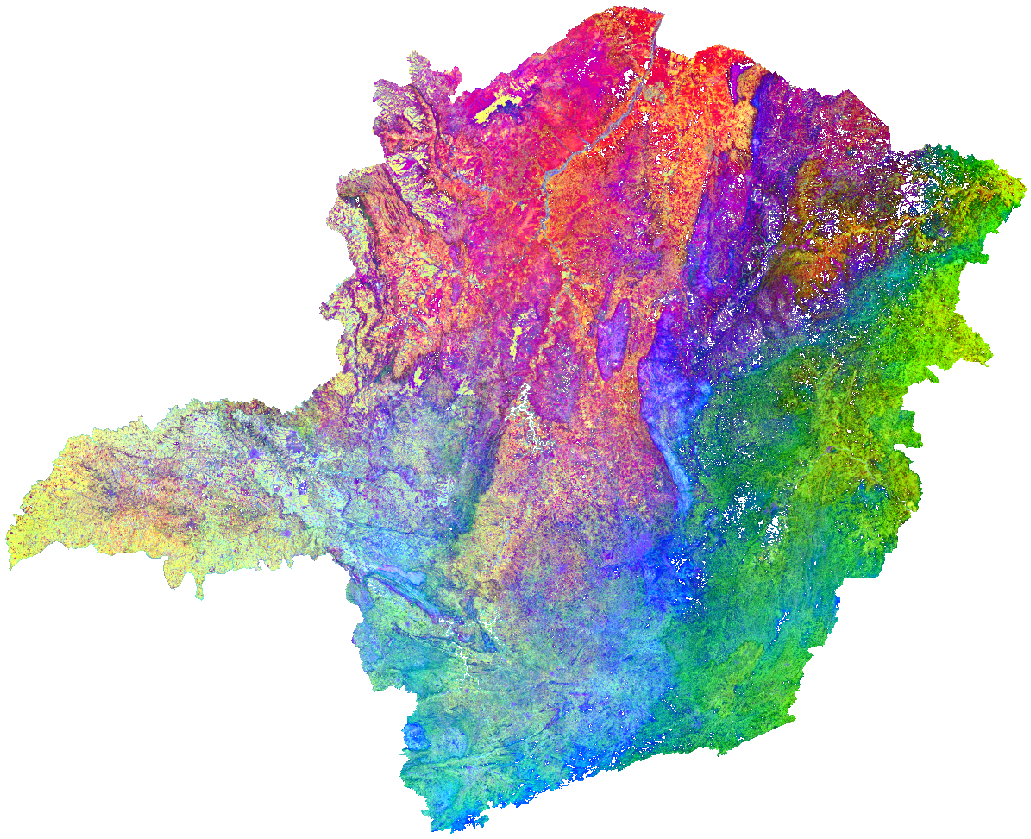
\includegraphics[height=0.74\paperheight]{hero_gsed.png}};
  \node[anchor=south east,draw=white,line width=1.5pt,inner sep=0] (tile) at ($(map.south east)+(0,-0.1)$)
    {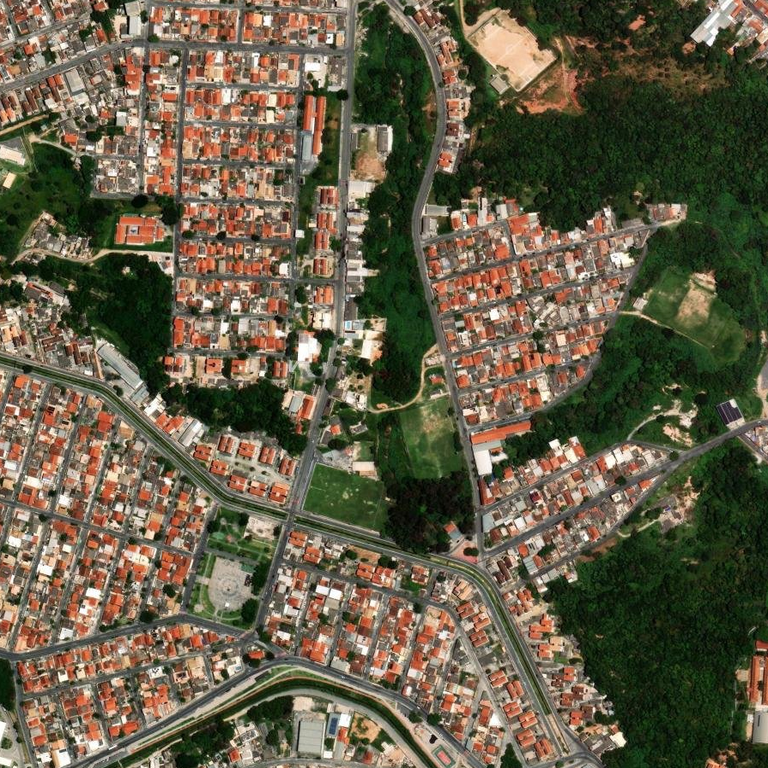
\includegraphics[width=2.3cm]{backup_tile4.png}};
  \node[anchor=north east,font=\tiny,text=muted,align=right] at (tile.south east)
    {one 1\,km cell, as the captioning model sees it};
  \node[anchor=north west,text width=6.2cm,align=left] at ($(current page.north west)+(0.7,-1.3)$) {
    {\color{accentdark}\Large\bfseries Estimating municipal GDP from satellite embeddings, text and night lights\par}
    \vspace{0.35cm}
    {\color{muted}\small Combining UrbanCLIP-style captions with night-light steering of Google satellite embeddings,
     tested on the \nMunis{} municipalities of Minas Gerais, Brazil\par}
    \vspace{0.6cm}
    {\small\bfseries Hemant\par}
    {\small\color{muted} Term project \textbullet\ mid-term review \textbullet\ October 2026\par}};
  \node[anchor=south west,font=\tiny,text=muted,align=left] at ($(current page.south west)+(0.7,0.3)$)
    {Map: first three principal components of the 64 GSED embedding bands, 1\,km cells};
\end{tikzpicture}
\end{frame}}

% ==== 2. Problem ============================================================
\begin{frame}{Official GDP is patchy below the national level --- satellites see everywhere}
\begin{columns}[T,onlytextwidth]
\column{0.42\textwidth}
\vspace{0.4cm}
\begin{itemize}
  \item Sub-national GDP is published late, estimated from partial data, or missing in many countries
  \item Satellites measure every place, every year, with the same sensor: an independent signal of economic activity
  \item \alert{Goal:} estimate municipal GDP per capita from free satellite data, and measure honestly how well it works
\end{itemize}
\vspace{0.3cm}
{\small\muted{Minas Gerais: richer agribusiness and mining south-west, poorer north-east --- a 50$\times$ range in GDP per capita.}}
\column{0.55\textwidth}
\centering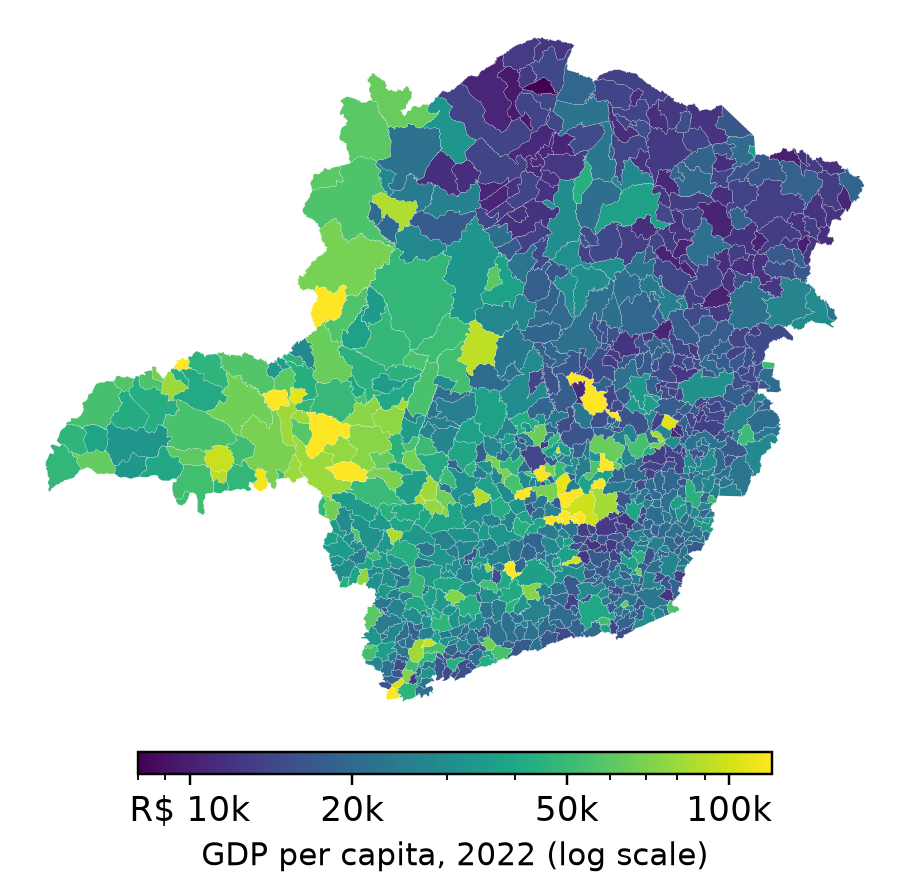
\includegraphics[height=6.4cm]{map_gdp.png}\\
{\scriptsize\muted{Official 2022 GDP per capita (IBGE), \nMunis{} municipalities}}
\end{columns}
\end{frame}

% ==== 3. Two ideas ==========================================================
\begin{frame}{We combine two recent ideas that have never been tested together}
\centering
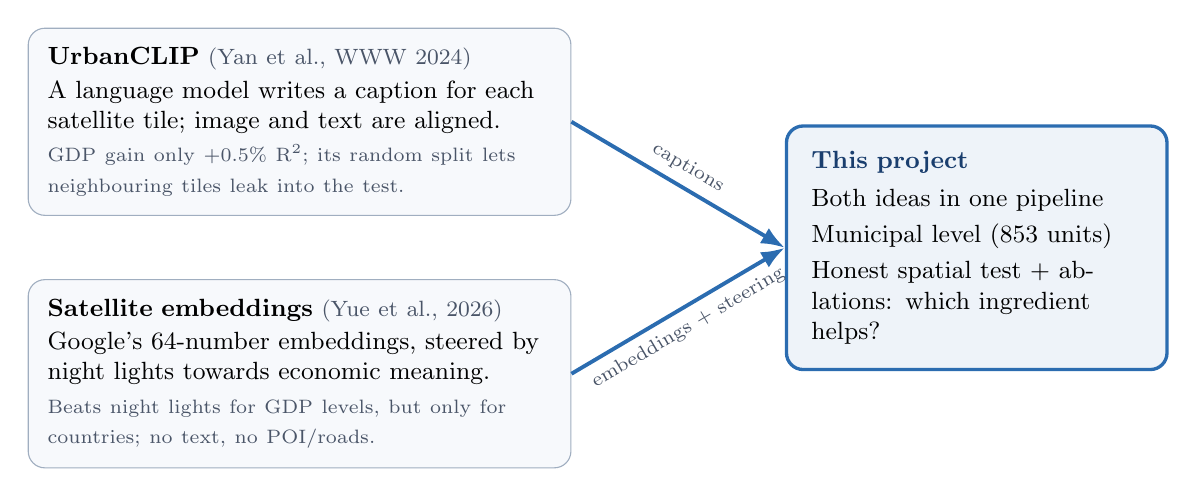
\begin{tikzpicture}[
  paper/.style={draw=softgrey,fill=paper,rounded corners=6pt,text width=6.4cm,inner sep=7pt,align=left,font=\small},
  ours/.style={draw=accent,line width=1.2pt,fill=accent!8,rounded corners=6pt,text width=4.2cm,inner sep=9pt,align=left,font=\small},
  arr/.style={-{Latex[length=3mm]},line width=1.4pt,color=accent}]
  \node[paper] (u) at (0,1.6) {{\bfseries UrbanCLIP} \muted{\footnotesize(Yan et al., WWW 2024)}\\[1pt]
    A language model writes a \alert{caption for each satellite tile}; image and text are aligned.\\[1pt]
    {\scriptsize\muted{GDP gain only +0.5\% R\textsuperscript{2}; its random split lets neighbouring tiles leak into the test.}}};
  \node[paper] (e) at (0,-1.6) {{\bfseries Satellite embeddings} \muted{\footnotesize(Yue et al., 2026)}\\[1pt]
    Google's \alert{64-number embeddings}, \alert{steered by night lights} towards economic meaning.\\[1pt]
    {\scriptsize\muted{Beats night lights for GDP levels, but only for countries; no text, no POI/roads.}}};
  \node[ours] (o) at (8.6,0) {{\bfseries\color{accentdark} This project}\\[3pt]
    Both ideas in one pipeline\\[2pt]
    Municipal level (\nMunis{} units)\\[2pt]
    Honest spatial test + ablations: which ingredient helps?};
  \draw[arr] (u.east) -- node[above,sloped,font=\scriptsize,text=muted]{captions} (o.west);
  \draw[arr] (e.east) -- node[below,sloped,font=\scriptsize,text=muted]{embeddings + steering} (o.west);
\end{tikzpicture}
\end{frame}

% ==== 4. Pipeline ===========================================================
\begin{frame}{The pipeline: three learning stages, from no labels to official GDP}
\centering
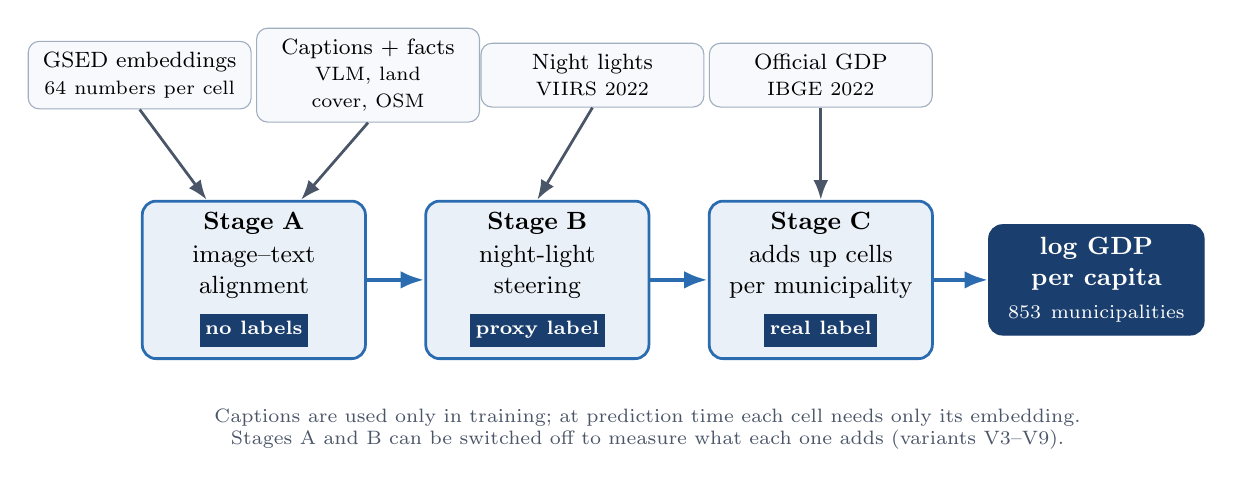
\begin{tikzpicture}[
  inp/.style={draw=softgrey,fill=paper,rounded corners=4pt,text width=2.55cm,align=center,font=\footnotesize,inner sep=4pt},
  stage/.style={draw=accent,fill=accent!10,line width=1pt,rounded corners=5pt,text width=2.6cm,align=center,
    minimum height=2.0cm,font=\small},
  arr/.style={-{Latex[length=2.5mm]},line width=1pt,color=muted},
  sarr/.style={-{Latex[length=3mm]},line width=1.6pt,color=accent}]
  \node[stage] (A) at (0,0) {{\bfseries Stage A}\\[1pt]image--text alignment\\[4pt]\chip{accentdark}{no labels}};
  \node[stage] (B) at (3.6,0) {{\bfseries Stage B}\\[1pt]night-light steering\\[4pt]\chip{accentdark}{proxy label}};
  \node[stage] (C) at (7.2,0) {{\bfseries Stage C}\\[1pt]adds up cells per municipality\\[4pt]\chip{accentdark}{real label}};
  \node[draw=accentdark,fill=accentdark,text=white,rounded corners=5pt,text width=2.5cm,align=center,
    minimum height=1.4cm,font=\small\bfseries] (Y) at (10.7,0) {log GDP\\per capita\\[1pt]\mdseries\scriptsize\nMunis{} municipalities};
  \node[inp] (g) at (-1.45,2.6) {GSED embeddings\\\scriptsize 64 numbers per cell};
  \node[inp] (t) at (1.45,2.6) {Captions + facts\\\scriptsize VLM, land cover, OSM};
  \node[inp] (n) at (4.3,2.6) {Night lights\\\scriptsize VIIRS 2022};
  \node[inp] (y) at (7.2,2.6) {Official GDP\\\scriptsize IBGE 2022};
  \draw[arr] (g.south) -- ($(A.north)+(-0.6,0)$);
  \draw[arr] (t.south) -- ($(A.north)+(0.6,0)$);
  \draw[arr] (n.south) -- (B.north);
  \draw[arr] (y.south) -- (C.north);
  \draw[sarr] (A) -- (B); \draw[sarr] (B) -- (C); \draw[sarr] (C) -- (Y);
  \node[font=\scriptsize,text=muted,text width=11cm,align=center] at (5,-1.9)
    {Captions are used only in training; at prediction time each cell needs only its embedding.\\
     Stages A and B can be switched off to measure what each one adds (variants V3--V9).};
\end{tikzpicture}
\end{frame}

% ==== 5. Data ===============================================================
\begin{frame}{We built a 1\,km dataset covering all \nMunis{} municipalities of Minas Gerais}
\begin{columns}[c,onlytextwidth]
\column{0.73\textwidth}
\centering
\thumb{thumb_gsed.png}{Satellite embeddings}{Google GSED, 10\,m $\to$ 1\,km}\hfill
\thumb{thumb_ntl.png}{Night lights}{VIIRS 2022}\hfill
\thumb{thumb_built.png}{Built-up land}{ESA WorldCover}\\[8pt]
\thumb{thumb_roads.png}{Roads and POIs}{OpenStreetMap}\hfill
\thumb{thumb_buildings.png}{Building footprints}{Microsoft + OSM}\hfill
\thumb{thumb_gdp.png}{GDP and population}{IBGE 2022 (target)}
\column{0.24\textwidth}
\bignum{\nMunis}{municipalities}\\[6pt]
\bignum{\nCells}{1\,km cells}\\[6pt]
\bignum{\nCaptions}{captioned tiles}\\[6pt]
\bignum{\nBuildings}{building footprints}
\end{columns}
\vspace{4pt}
{\scriptsize\muted{All layers are free and share one 1\,km grid. The GDP target is official statistics, not derived from night lights.}}
\end{frame}

% ==== 6. Captions ===========================================================
\begin{frame}{A vision--language model describes each tile; data checks remove false claims}
\begin{columns}[T,onlytextwidth]
\column{0.36\textwidth}
\centering
\begin{tikzpicture}
  \node[inner sep=0] (im) {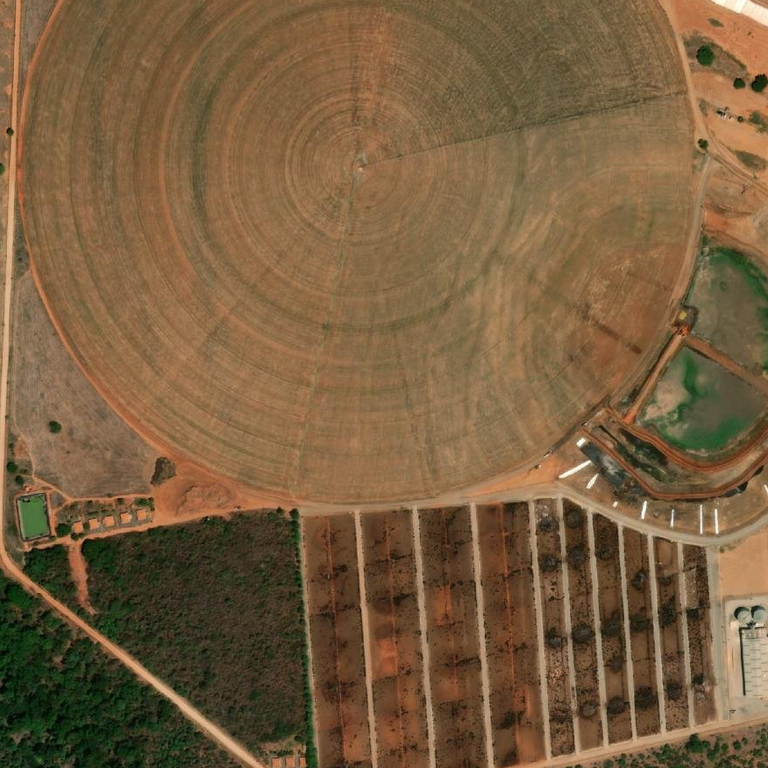
\includegraphics[width=0.84\linewidth]{caption_tile.png}};
  % image-relative coordinates: (0,0) bottom left, (1,1) top right
  \begin{scope}[x={($(im.south east)-(im.south west)$)},y={($(im.north west)-(im.south west)$)},shift={(im.south west)}]
    \draw[dropc,line width=1.3pt,dashed] (0.43,0.64) ellipse (0.36 and 0.33);
    \node[anchor=south west,font=\scriptsize,fill=white,fill opacity=0.88,text opacity=1,text=dropc,inner sep=2pt]
      at (0.02,0.02) {centre-pivot irrigation, not a mine};
  \end{scope}
\end{tikzpicture}\\[1pt]
{\scriptsize\muted{Esri World Imagery, \textasciitilde1\,m per pixel}}\\[5pt]
\chip{accent}{\nCaptions{} captions}\ \chip{done}{\nKept{} of sentences kept}\\[3pt]
\chip{running}{blind hand audit in progress}
\column{0.6\textwidth}
{\small\bfseries Qwen2.5-VL-7B caption}\ {\footnotesize\muted{after data checks}}\\[-2pt]
\begin{itemize}\setlength{\itemsep}{0pt}\footnotesize
\dropped{The satellite image shows a large circular area with concentric rings, likely a mine pit, surrounded by a grid of smaller rectangular plots of farmland.}{unsupported industry claim}
\keep{Roads crisscross the area, connecting the plots and the perimeter.}
\keep{Vegetation is sparse, mostly along the edges and in some patches within the farmland.}
\keep{A small body of water, possibly a pond, is visible near the farmland.}
\keep{No buildings or industrial structures are evident, suggesting minimal built-up area.}
\dropped{The overall scene appears to be an agricultural landscape with a focus on farming and possibly mining operations.}{filler}

\end{itemize}
\end{columns}
\end{frame}

% ==== 7. Evaluation =========================================================
\begin{frame}{Every municipality is tested in a region the model never saw}
\begin{columns}[c,onlytextwidth]
\column{0.5\textwidth}
\centering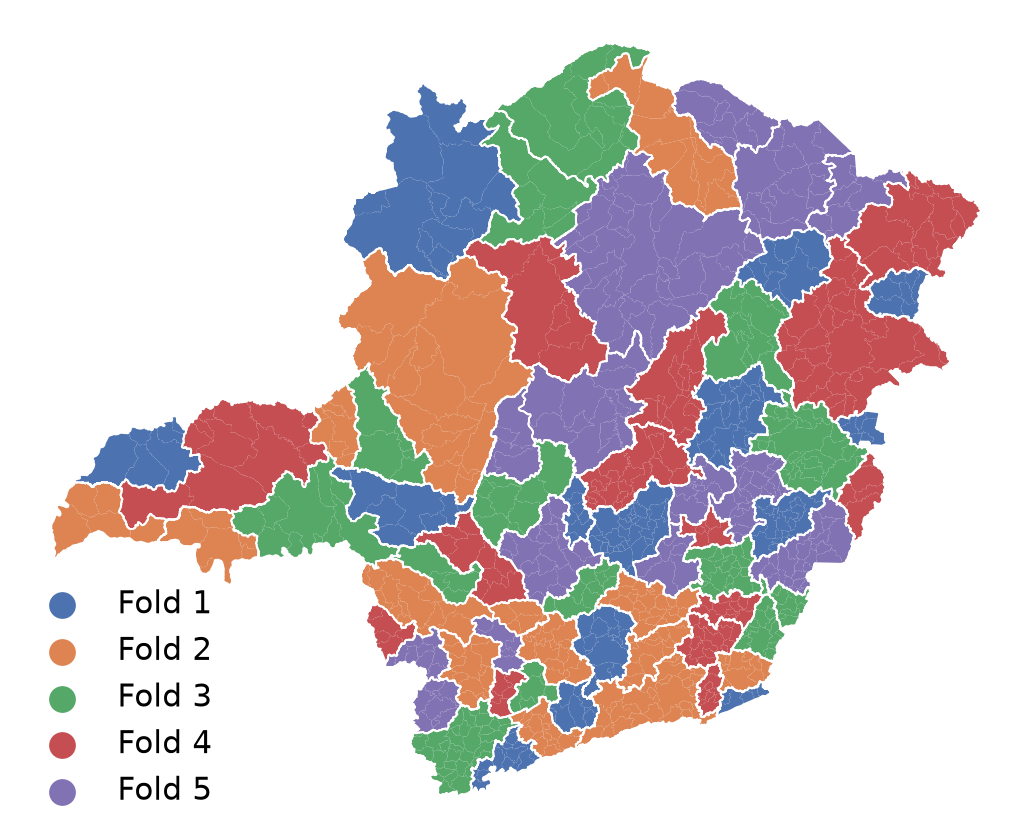
\includegraphics[height=6.3cm]{map_folds.png}
\column{0.47\textwidth}
\begin{itemize}
  \item 70 official regions of neighbouring municipalities $\to$ 5 balanced folds
  \item Each round: 3 folds train, 1 validates, \alert{1 is tested}; all stages are retrained
  \item Nearby places look alike, so holding out whole regions prevents the leakage in UrbanCLIP's random split
\end{itemize}
\vspace{0.3cm}
{\small\muted{Differences between models are tested with a block bootstrap over regions (95\% intervals).}}
\end{columns}
\end{frame}

% ==== 8. Results ============================================================
\begin{frame}{First results: the hybrid model explains about half of GDP variation}
\begin{columns}[c,onlytextwidth]
\column{0.64\textwidth}
\centering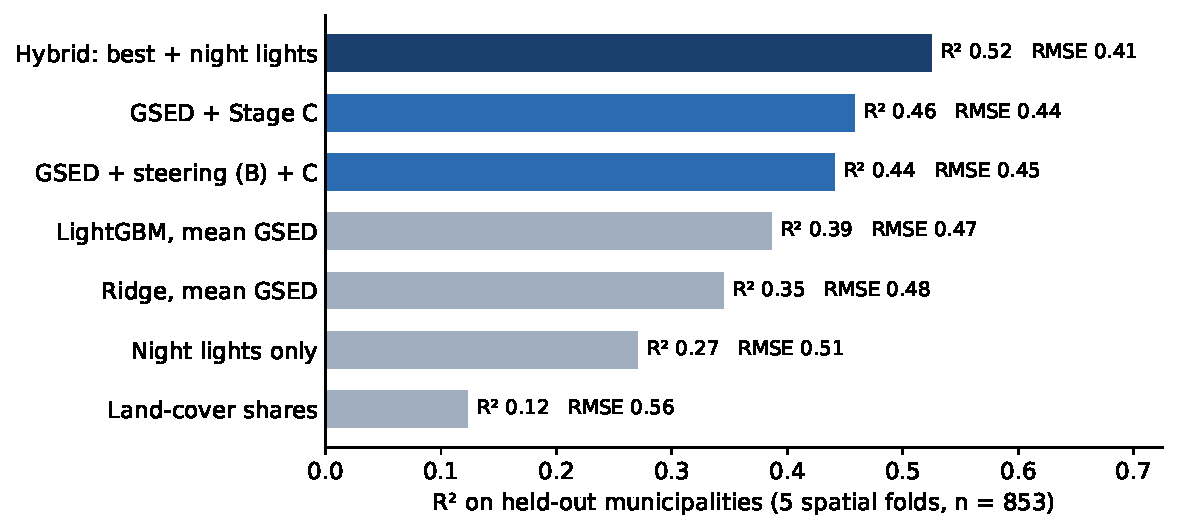
\includegraphics[width=\linewidth]{chart_results.pdf}
\column{0.33\textwidth}
{\small\color{accent}\rule{6pt}{6pt}} {\scriptsize our pipeline}\quad
{\small\color{softgrey}\rule{6pt}{6pt}} {\scriptsize baselines}\\[10pt]
{\small\bfseries RQ1} \chip{nextc}{steering}\\
{\scriptsize\RQone}\\[8pt]
{\small\bfseries RQ4} \chip{done}{hybrid}\\
{\scriptsize\RQfour}\\[8pt]
{\small\bfseries RQ2, RQ3} \chip{running}{text, POI/roads}\\
{\scriptsize text variants V5--V9 finishing now}
\end{columns}
\vspace{2pt}
{\scriptsize\muted{Night lights alone: R\textsuperscript{2} \nNtlR{}. Hybrid = our best model blended with the night-light benchmark (weight chosen on validation).}}
\end{frame}

% ==== 9. Lessons ============================================================
\begin{frame}{Lessons so far: calibration mattered more than night-light steering}
\begin{columns}[c,onlytextwidth]
\column{0.45\textwidth}
\centering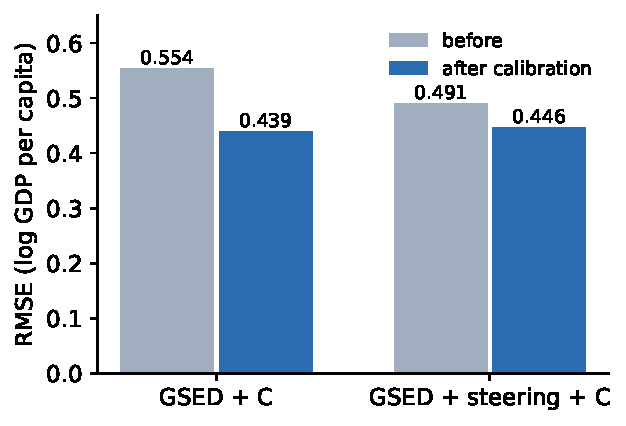
\includegraphics[width=\linewidth]{chart_calibration.pdf}\\
{\scriptsize\muted{Same models, before and after a validation-fitted correction}}
\column{0.52\textwidth}
\begin{enumerate}\setlength{\itemsep}{6pt}
  \item \textbf{Predictions were over-spread.} A straight-line correction fitted on validation municipalities cut error by about 20\%.
  \item \textbf{Honest testing changes conclusions.} Steering looked helpful before the fix; after it, the gain vanished.
  \item \textbf{Captions need checking.} The model invents mines, roads and farmland on featureless tiles; data checks remove most of it.
\end{enumerate}
\end{columns}
\end{frame}

% ==== 10. Progress ==========================================================
\begin{frame}{About 80\% done: text experiments are finishing, full results this week}
\begin{columns}[T,onlytextwidth]
\column{0.56\textwidth}
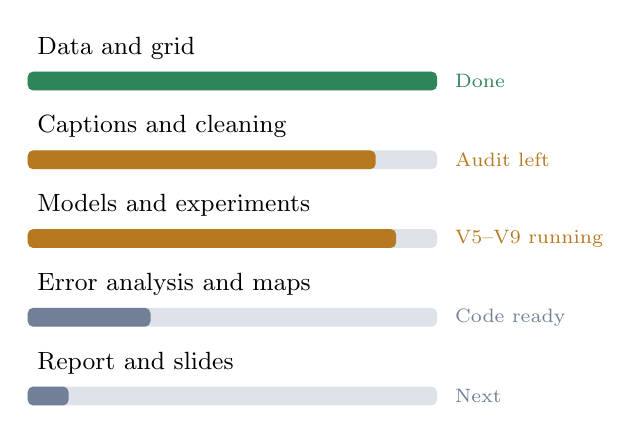
\begin{tikzpicture}[x=5.2cm,y=1.0cm]
  \foreach \lab/\pct/\fc/\st [count=\i] in {
      Data and grid/1.00/done/Done,
      Captions and cleaning/0.85/running/Audit left,
      Models and experiments/0.90/running/V5--V9 running,
      Error analysis and maps/0.30/nextc/Code ready,
      Report and slides/0.10/nextc/Next} {
    \node[anchor=west,font=\small] at (0,-\i+0.22) {\lab};
    \fill[softgrey!35,rounded corners=2pt] (0,-\i-0.08) rectangle (1,-\i-0.32);
    \fill[\fc,rounded corners=2pt] (0,-\i-0.08) rectangle (\pct,-\i-0.32);
    \node[anchor=west,font=\scriptsize,text=\fc] at (1.02,-\i-0.2) {\st};
  }
\end{tikzpicture}
\column{0.4\textwidth}
{\small\bfseries Research questions}\\[4pt]
\renewcommand{\arraystretch}{1.25}
\begin{tabular}{@{}l l@{}}
\small RQ1 steering & \chip{done}{answered}\\
\small RQ2 text & \chip{running}{running}\\
\small RQ3 POI and roads & \chip{running}{running}\\
\small RQ4 hybrid & \chip{done}{answered}\\
\small RQ5 where it fails & \chip{nextc}{next}\\
\end{tabular}\\[10pt]
{\small\bfseries Next}\\[2pt]
{\small text results $\to$ caption audit $\to$ error analysis and 1\,km maps $\to$ report}
\end{columns}
\end{frame}

% ==== Backup ================================================================
\appendix
\begin{frame}{Backup: data sources}
\footnotesize
\renewcommand{\arraystretch}{1.15}
\begin{tabularx}{\textwidth}{@{}p{3.1cm} p{6.0cm} >{\raggedright\arraybackslash}X@{}}
\toprule
Layer & Source & Use \\
\midrule
Satellite embeddings & Google Satellite Embedding V1 (AlphaEarth), 2022 & image input, averaged 10\,m $\to$ 1\,km \\
Night lights & VIIRS DNB annual V2.2, 2022 & Stage B proxy label, night-light benchmark \\
Land cover & ESA WorldCover v200, 2021 & masking, fact sentences, caption checks \\
Roads, POIs & OpenStreetMap (Geofabrik, 2023-01-01) & features, fact sentences, caption checks \\
Buildings & Microsoft ML footprints + OSM & caption checks \\
Caption imagery & Esri World Imagery (ArcGIS Location Platform) & input to the vision--language model \\
GDP, population & IBGE municipal GDP 2022, Census 2022 & target (log GDP per capita) \\
\bottomrule
\end{tabularx}
\end{frame}

\begin{frame}{Backup: Stage A aligns embeddings and captions far above chance}
\begin{columns}[c,onlytextwidth]
\column{0.5\textwidth}\centering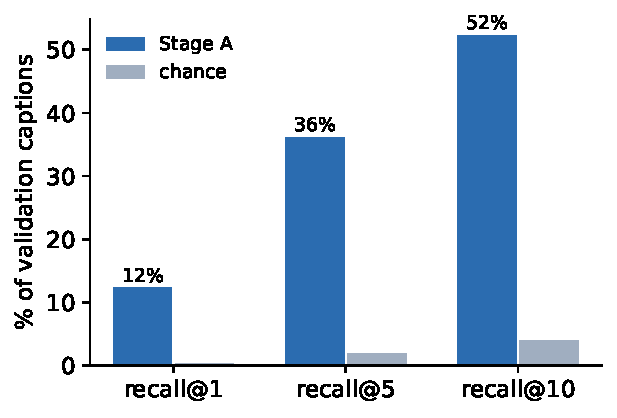
\includegraphics[width=\linewidth]{chart_recall.pdf}
\column{0.45\textwidth}
\small For a validation tile, how often is its own caption among the top $k$ of 256 candidates?\\[6pt]
\muted{Part of the alignment comes from the fact sentences; variants V8 (captions only) and V9 (facts only) separate the two.}
\end{columns}
\end{frame}

\begin{frame}{Backup: what the captions look like}
\bt{backup_tile1.png}{\bcapnameA}{\bcapA}\hfill
\bt{backup_tile2.png}{\bcapnameB}{\bcapB}\hfill
\bt{backup_tile3.png}{\bcapnameC}{\bcapC}\hfill
\bt{backup_tile4.png}{\bcapnameD}{\bcapD}
\vspace{6pt}

{\scriptsize\muted{First sentence of each caption that passed the cleaning checks.}}
\end{frame}

\end{document}
